\documentclass[aps, reprint,amsmath,amssymb]{revtex4-1} %APS Journal
\usepackage[T1]{fontenc}
\usepackage[utf8]{inputenc}
\usepackage{lmodern}
\usepackage{microtype}
\usepackage{graphicx}
\usepackage{siunitx}
\usepackage{bm}

\renewcommand{\vec}[1]{\boldsymbol{#1}}
\newcommand{\mat}[1]{\mathbf{#1}}
\newcommand{\uv}[1]{\vec{\hat{#1}}}
\newcommand{\x}{\vec{\hat{x}}}
\newcommand{\y}{\vec{\hat{y}}}
\newcommand{\z}{\vec{\hat{z}}}
\renewcommand{\d}{\partial}
\renewcommand{\L}{\mathcal{L}}
\renewcommand{\inf}{\infty}

\begin{document}
%----------------------------------------------------------------------
% title
%----------------------------------------------------------------------
\title{PHY64 Experiment 3: The Frank-Hertz Experiment}
\author{Matthew S. E. Peterson}
\author{Jackson Burzynski}
\affiliation{Department of Physics and Astronomy, Tufts University}
%\date{\today} 
\maketitle

%----------------------------------------------------------------------
% Body
%----------------------------------------------------------------------
\section{Introduction}
In 1914 German physicists James Frank and Gustav Hertz performed the first measurement to clearly show the quantum nature of atoms. By bombarding gases with energetic electrons, Frank and Hertz observed that the transfer of kinetic energy from an electron could raise a mercury atom from its ground state to an excited state. The pair discovered that when an electron collided with a mercury atom, it could lose only a specific amount of its kinetic energy. Frank and Hertz were able to show that atoms absorb kinetic energy from electrons in quantized amounts. In a later experiment, they showed that the exited atoms radiate away the absorbed energy in these same amounts.

We replicate the Frank-Hertz experiment with an apparatus similar to the one used by Frank and Hertz in 1914. The central element of our experiment is a tube manufactured by Klinger consisting of three electrodes. The tube is evacuated except for the presence of a small amount of mercury. The cathode is heated by a filament to emit electrons. The electrons are then accelerated to the anode by a potential difference $V_a$. The anode is a mesh to allow for energetic electrons to pass through and reach the repeller. The repeller potential $V_r$ is set to be negative relative to the anode so that only electrons with kinetic energy greater than $eV_r$ may reach the repeller. The current $I$ formed by the electrons reaching the repeller is measured by a picoameter. The collisions between electrons and mercury atoms result in a periodic variation of the repeller current. From the periodicity of this current we may infer the energy of the first excited state of the mercury atom.

\section{Theory}

When the accelerating voltage $V_a$ is small, the collisions between the electrons and the mercury atoms are completely elastic. As $V_a$ is increased, a threshold voltage is reached in which inelastic collisions between the electrons and the mercury atoms begin to occur. In these collisions, the electrons transfer almost of of their kinetic energy to the atom, causing a transition from the ground state to the first excited state. The electrons that have lost their kinetic energy in these collisions are then unable to reach the repeller, resulting in a decrease in the current $I$. As we continue to increase $V_a$, the scattered electrons are reaccelerated and are capable of overcoming the retarding current and reach the repeller resulting in an increase in the current. The current continues to increase until $V_a$ is large enough for an electron to have two inelastic collisions. As in the single-scattering scenario, these electrons have insufficient energy to reach the repeller, resulting in second decrease in the current $I$. This phenomenon continues as $V_a$ is increased to allow for higher collision multiplicities. By observing the locations of the current peaks we may deduce the magnitude of the first excited state of the mercury atom

\section{Results}

We vary the voltage $V_a$ from zero to 30 V to determine the positions of the current peaks. The current variations are recorded through an oscilloscope and are shown in figures~\ref{fig:160} and ~\ref{fig:152}
\begin{figure}
\centering
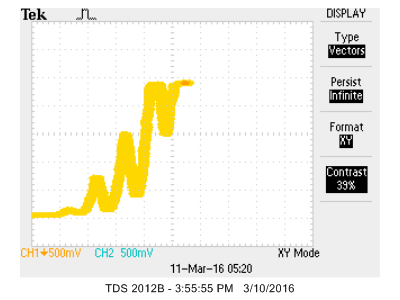
\includegraphics[width=8cm]{jb_mp_152.png}
\caption{Current variation at 152K}
\label{fig:152}
\end{figure}

\begin{figure}
\centering
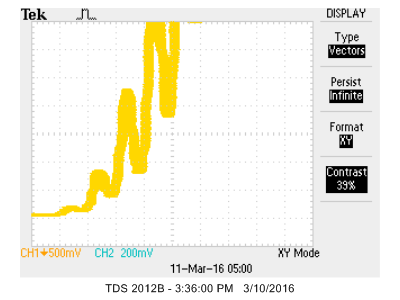
\includegraphics[width=8cm]{jb_mp_160.png}
\caption{Current variations at 160K}
\label{fig:160}
\end{figure}

Several trials were performed at different temperatures for more accurate results. The periodicity of the current variations is obtained by observing the voltage difference between local maxima. These periodicities are averaged over all trials performed to obtain a more accurate measurement. The average periodicity is calculated to be
\[
	V =  \SI{4.946}{V}
\]
Hence, from this we deduce that the energy of the first excited state of the mercury atom is
\[
	E_1 =  \SI{4.946}{eV}
\]
There is an offset to the pattern of voltages at which the current reaches its local maxima. This is due to the presence of a contact potential generated by the two different metals used in the fabrication of the cathode and anode in our apparatus. This offset is observed to be 
\[
	V_c = \SI{2.063}{V}.
\]

\section{Error}

The width of the local maxima in the oscilloscope data give rise to a proportional amount of uncertainty in our measurement. The exact position of the maximum is difficult to ascertain given the large number of points on the oscilloscope curves corresponding to the same maximal current values. Thus, each measured interval between successive local maxima is assigned a relative uncertainty. Using the error propagation formula we, calculate a value for the overall uncertainty in our measurement. The standard deviation of the measurement of $E_1$ is found numerically to be
\[
    \sigma_{E_1} = \SI{0.173}{eV}.
\]
Similarly, the error in our result for the contact potential is calculated to be
\[
    \sigma_{V_c} = \SI{0.173}{eV}.
\]

\section{Conclusion}
We were able to calculate the value of $E_1$ to be
\[
    E = (4.946 \pm 0.173) \si{eV}.
\]
Comparing this with the known value of the first excited state of mercury, $E_1 = \SI{4.9}{eV}$, we see that the known value of $E_1$ falls within one standard deviation of our measurement. Thus, our experimentally determined value of $E_1$ agrees reasonably with the
known value. The exact value for the contact potential in our apparatus is not known, but our measured value of 
\[
    V_c = (2.063 \pm 0.155) \si{V}.
\]
is consistent with our expectations.

\end{document}
